\documentclass[11pt]{article}
\usepackage[a4paper,margin=24mm]{geometry}
\usepackage[T1]{fontenc}
\usepackage[utf8]{inputenc}
\usepackage{lmodern,microtype}
\usepackage{amsmath,amssymb,amsthm,mathtools}
\usepackage{booktabs,longtable,array,tabularx}
\usepackage{enumitem,xcolor,graphicx}
\usepackage{listings}
\usepackage[colorlinks=true,linkcolor=blue!45!black,citecolor=blue!45!black,urlcolor=blue!45!black]{hyperref}
\hypersetup{pdftitle={Exact symbolic compression for unknot recognition},pdfauthor={ProveIt research continuation}}
\setlength{\parskip}{4pt}
\setlength{\parindent}{0pt}
\setlist{nosep,leftmargin=*}
\emergencystretch=2em
\newtheorem{theorem}{Theorem}[section]
\newtheorem{proposition}[theorem]{Proposition}
\newtheorem{lemma}[theorem]{Lemma}
\newtheorem{corollary}[theorem]{Corollary}
\theoremstyle{definition}
\newtheorem{definition}[theorem]{Definition}
\theoremstyle{remark}
\newtheorem{remark}[theorem]{Remark}
\newcommand{\F}{\mathbb F_2}
\newcommand{\Kh}{\widetilde{\operatorname{Kh}}}
\newcommand{\rank}{\operatorname{rank}}
\newcommand{\im}{\operatorname{im}}
\newcommand{\id}{\operatorname{id}}
\newcommand{\poly}{\operatorname{poly}}
\newcommand{\bits}{\operatorname{bits}}
\newcommand{\code}[1]{\texttt{#1}}
\lstset{basicstyle=\ttfamily\small,breaklines=true,columns=fullflexible,keepspaces=true,frame=single,rulecolor=\color{black!15},showstringspaces=false}

\title{Exact symbolic compression for unknot recognition:\\
graded transfer, finite twist tails, and the remaining complexity barrier}
\author{ProveIt research continuation}
\date{7--8 October 2026}

\begin{document}
\maketitle
\begin{abstract}
We continue the implementation and mathematical analysis of the ProveIt unknot recognizer against the current integrated source, rather than an earlier research archive. The main algebraic result is an exact transfer algorithm for a partially reduced Bar--Natan complex. Its scalar differential is contracted by binary linear algebra, and every surviving non-scalar map is recovered by a finite pass through the quantum grading. This removes the common-disk assumption from the termination argument for this particular transfer and handles consecutive surviving homological degrees with nonzero differentials. The second result is an effective finite-tail formula for one long signed braid twist in an arbitrary fixed context. If the other runs contain $L$ crossings, a calculation at exponent magnitude $L+2$ determines a compact full homological-degree profile for every longer exponent; the total-rank formula already begins at $L+1$. The resulting bound depends exponentially on $L$ and only polynomially on the binary input length. We derive and delimit a dominance obstruction, including its subsumption by the existing Seifert certificate. A succinct signed-run front end avoids expanding large exponents for those certificates. Independent chain identities, exact comparisons, resource tests, and paired timings accompany the code. Finally, we give a repair-dependency bound for a prospective geometric hierarchy algorithm. No general quasi-polynomial bound for unknot recognition is proved: surviving state volume, representation growth, and constructive repair dependencies remain uncontrolled.
\end{abstract}

\clearpage
\tableofcontents
\newpage

\section{Outcome, baseline, and scope}
\label{sec:scope}

\subsection{What this installment changes}
The maintained Python implementation already contains substantially more than its original scanning engine. The baseline for this report is ProveIt commit
\begin{center}
\code{d54009df0ea3751b8662bb76549d3c1bb0eec19c}.
\end{center}
Its commit timestamp is 8 October 2026, 01:20:13 UTC. We retrieved the active \path{Topology/UnknotRecognition/fast/} tree, the synthesis sources, and the recent report summaries through the GitHub connector. All 114 retrieved text files were checked against their Git blob identifiers. The active baseline passes 245 tests in this environment; the retained log records 37.786 seconds. These observations describe this snapshot, not a later upstream branch.

The starting implementation includes complete recognition of source braids on at most three strands; signed Seifert-graph certificates; checked visible-sum decomposition; Alexander and Jones filters; exact standard, shared, and twist-compressed Khovanov backends; componentwise coefficient contraction; scalar-residue survivor prediction; adaptive cancellation; and exact homological windows. The synthesis already records why a small frontier or inexpensive coefficient multiplication alone does not control the number of chain objects. These are inherited results, not contributions claimed here \cite{proveit}.

The work below addresses three specific interfaces where an exponential or numerically large representation was still being expanded:
\begin{enumerate}
\item Scalar cancellation can determine the surviving objects cheaply, but an exact continuation also needs the maps between them. We compute those maps by a grading-directed transfer.
\item A long two-strand twist contains a repeated homological interior. We replace the repeated output by a finite calculation and a symbolic interval.
\item A braid supplied by binary signed exponents need not be expanded to construct the signed Seifert graph. We evaluate its structural certificates directly.
\end{enumerate}
The first two are mathematically distinct. The transfer is a relative-boundary equivalence usable before further gluing; the twist formula computes the homology of a specified closed braid and must not be treated as a relative tangle replacement.

\subsection{Claim ledger}
\begin{center}
\begin{tabularx}{\textwidth}{@{}>{\raggedright\arraybackslash}p{0.24\textwidth}>{\raggedright\arraybackslash}X>{\raggedright\arraybackslash}p{0.23\textwidth}@{}}
\toprule
Result & What is established & Limitation \\
\midrule
Graded transfer & Full transferred differential and chain-contraction identities; finite evaluation by increasing quantum shift & Object multiplicities and binary matrix sizes remain parameters \\
Finite twist tail & Exact total rank and compact homological-degree profile from a finite cap & One selected long run; quantum grading is forgotten \\
Succinct certificates & Exact structural decisions directly on binary signed runs & Inconclusive inputs still need the complete backend \\
Repair dependency & Explicit weighted-path bound for a certified acyclic dependency graph & No universal suitable graph is constructed for knot exteriors \\
General recognition & Sound complete fallback when resource caps are removed & No $n^{O(\log n)}$ worst-case bound \\
\bottomrule
\end{tabularx}
\end{center}

\subsection{Input sizes and recognition semantics}
Let $n$ be the number of explicitly listed crossings or braid letters. For a signed-run input
\[
 \beta=\sigma_{i_1}^{e_1}\cdots\sigma_{i_t}^{e_t},\qquad e_j\ne0,
\]
let $b$ denote the strand count and let $N$ denote its binary encoding length. In particular $n=\sum_j|e_j|$ can be exponential in $N$. Every complexity assertion specifies which size is used. A compact homology profile and an expanded list of its coefficients are different outputs: writing a nonzero coefficient in each of $m$ degrees already costs $\Omega(m)$ output operations.

The recognizer accepts only a one-component classical knot for an unknot decision. A braid word defines a classical closure automatically, and its component count is the cycle count of the strand permutation. A partial calculation, a failed certificate search, or a resource exception never certifies triviality. Exact reduced $\F$-Khovanov rank one detects the unknot: the rational detection theorem of Kronheimer--Mrowka and universal coefficients give the required implication over $\F$; the unknot has rank one over $\F$ directly \cite{km}. The computation below does not replace that theorem by finite testing.

\section{The grading makes exact transfer triangular}
\label{sec:graded}

\subsection{Typed morphisms and their intrinsic weight}
At a scan frontier with $2k$ endpoints, a chain object is a perfect matching $a$ together with a homological degree $h$ and a quantum shift $q$. Write $c(a,b)$ for the number of circles in the overlay of two matchings. A basis cobordism $x_S:a\to b$ has a dot on the components in $S$. In the conventions of the current scanner its intrinsic weight is
\begin{equation}
 \omega(x_S)=k-c(a,b)+2|S|.
 \label{eq:weight}
\end{equation}
The standard dotted grading in Bar--Natan's category gives, for every nonzero term of a differential entry $a_u\to a_v$,
\begin{equation}
 q_v-q_u=\omega(x_S).
 \label{eq:q}
\end{equation}
The synthesis established this convention and audited it numerically. The new implementation retains the shifts that were previously only a diagnostic. Starting with $q=0$, smoothing $i\in\{0,1\}$ and delooping $c$ circles with label $\ell$ gives
\begin{equation}
 q'=q+i+c-2\operatorname{popcount}(\ell).
 \label{eq:qrec}
\end{equation}
This is aligned with the current object-allocation order. Quantum shifts are preserved under scalar identity cancellation. The full grading theory and local cancellation mechanism are standard \cite{barnatan,fastkh}; the contribution here is their use in the concrete transfer algorithm.

\begin{lemma}[Zero weight]
Every weight in \eqref{eq:weight} is nonnegative. Weight zero occurs precisely for the undotted identity between equal matchings. The weight of every nonzero term of a composite is the sum of the input weights.
\end{lemma}
\begin{proof}
The overlay has at most $k$ circles. Equality means that every overlay component is a two-edge circle, hence that the two matchings agree. With equality, zero weight also requires no dots. Additivity follows from the cobordism degree, or directly from the Euler-characteristic relation used by the composition engine:
\[
2r=2u+2v+k-c(a,b)-c(b,c)+c(a,c)
\]
for input dot counts $u,v$ and output dot count $r$ on a surviving term. Substitution in \eqref{eq:weight} gives the asserted sum. Terms killed by the Frobenius relations make no contribution.
\end{proof}

Separate the differential as
\[
 d=d_0+\delta,
\]
where $d_0$ retains only weight-zero entries. Thus $d_0$ is a direct sum of ordinary binary complexes indexed by matching and quantum shift; $\delta$ strictly increases $q$. Equation $d^2=0$ implies $d_0^2=0$ by taking weight zero. Notice the typing condition: an undotted map between unequal matchings belongs to $\delta$, not to $d_0$.

\subsection{Constructing an actual scalar contraction}
A rank calculation alone does not suffice. We construct maps
\[
 I:H\longrightarrow C,\qquad P:C\longrightarrow H,\qquad
 H_0:C\longrightarrow C[-1]
\]
over scalar identities, satisfying
\begin{gather}
 PI=1,\quad d_0I=0,\quad Pd_0=0,\quad
 d_0H_0+H_0d_0=1+IP,\label{eq:contraction}\\
 H_0^2=0,\quad H_0I=0,\quad PH_0=0.\label{eq:side}
\end{gather}
All three maps preserve matching and quantum shift; $I,P$ preserve homological degree and $H_0$ lowers it by one. The plus sign in \eqref{eq:contraction} is appropriate in characteristic two.

For each fixed matching and $q$, choose in degree $h$ a basis $B^h$ of $\im d_0^{h-1}$, representatives $R^h$ complementing $B^h$ in $\ker d_0^h$, and lifts $L^h$ of a basis of $\im d_0^h$. Then
\[
 C^h=B^h\oplus R^h\oplus L^h,
\]
and $d_0$ maps $L^h$ isomorphically onto $B^{h+1}$. Inclusion and projection on $R^h$, together with the inverse $B^{h+1}\to L^h$, give \eqref{eq:contraction}--\eqref{eq:side}. Packed binary elimination constructs these bases and inverse coordinate maps. In particular, the algorithm knows the representatives and contractions, not only their dimensions.

\subsection{Finite transfer and its proof}
Let $r$ be the number of distinct quantum shifts among the live objects. Since $H_0$ preserves $q$ and $\delta$ strictly raises it, $(H_0\delta)^r=0$ and $(\delta H_0)^r=0$ as typed matrices. Define the finite sums
\[
 U=(1+H_0\delta)^{-1}=\sum_{j=0}^{r-1}(H_0\delta)^j,
 \qquad V=(1+\delta H_0)^{-1}=\sum_{j=0}^{r-1}(\delta H_0)^j.
\]

\begin{theorem}[Grading-directed exact transfer]
\label{thm:transfer}
For a valid finite graded scan complex, set
\begin{equation}
 D=P\delta UI,\qquad I'=UI,\qquad P'=PV,\qquad H'=UH_0=H_0V.
 \label{eq:hpl}
\end{equation}
Then $D^2=0$, and $(I',P',H')$ is a special chain contraction from $(C,d)$ onto $(H,D)$. In particular,
\begin{gather}
 dI'=I'D,\qquad P'd=DP',\qquad P'I'=1,\label{eq:newmaps}\\
 dH'+H'd=1+I'P',\qquad H'^2=0,\qquad H'I'=P'H'=0.\label{eq:newhomotopy}
\end{gather}
Every entry of $D$ has positive weight. The construction is valid for every matching frontier realized by the scanner; a common disk containing all matching diagrams is not an additional hypothesis.
\end{theorem}
\begin{proof}
Finite nilpotence was proved from the actual object shifts. Thus all displayed inverses are finite matrices over the same additive cobordism category. This is the basic perturbation identity, with a concrete terminating filtration \cite{real}. We give the algebraic checks needed here.

Write $Z=UI$. Its defining equation is $Z=I+H_0\delta Z$. Using \eqref{eq:contraction}, $d_0I=0$, and $d_0\delta+\delta d_0+\delta^2=0$ gives
\[
 dZ=ID+H_0\delta dZ.
\]
Multiplication by $U$ yields $dZ=ZD$. The corresponding right-hand calculation gives $P'd=DP'$. The identities $UH_0=H_0V$, $VH_0=H_0$, and $H_0U=H_0$ follow by expanding the finite sums and using $H_0^2=0$. Together with $H_0I=PH_0=0$, expansion proves $P'I'=1$, $H'I'=P'H'=H'^2=0$. Finally multiply $dH'+H'd+1+I'P'$ on the left by $1+H_0\delta$ and on the right by $1+\delta H_0$. Expanding, using $(d_0+\delta)^2=0$, and substituting $d_0H_0+H_0d_0=1+IP$ cancels every term. Both multipliers are invertible, proving the homotopy identity. From $dI'=I'D$ and $P'I'=1$ we obtain $D^2=P'd^2I'=0$. Each term of $D$ contains at least one $\delta$, so has positive weight. The proof uses the typed composition law and the finite grading, not a count of planar matching types.
\end{proof}

The theorem proves the finite nilpotence needed for the actual graded matrix calculation. It does not require a classification of ungraded frontier algebras or an interpretation of arbitrary formal matching tables as a common-disk arc algebra.

\subsection{Evaluate the sum without forming powers}
For a survivor basis vector $e$, the lifted column $Z=I'e$ solves
\begin{equation}
 Z=Ie+H_0W,\qquad W=\delta Z,\qquad De=PW.
 \label{eq:forward}
\end{equation}
Process quantum shifts in increasing order. Before a block of shift $q$ is processed, every contribution to $W_q$ has arrived from lower shifts. Compute $Z_q=(Ie)_q+(H_0W)_q$, propagate it along the outgoing $\delta$ entries, and accumulate the corresponding $P W_q$. No subsequent block can change this block. All equal-weight scalar mixing is confined to the already computed binary maps.

There is a useful additional finite band. Any nonzero basis morphism has
\[
 \omega=k-c(a,b)+2|S|\le k+c(a,b)\le 2k.
\]
Consequently a column whose source shift is $q_0$ cannot have a nonzero entry at a target shift greater than $q_0+2k$. The implementation discards such contributions before composing them. Equivalently, on these valid typed graded complexes, the weak bound $(H_0\delta)^{2k+1}=0$ also holds: a product containing more than $2k$ strictly positive-weight factors has no possible nonzero output monomial. This is a source-to-target weight argument; it does not assume that an arbitrary formal matching product is realized by a valid scan. The forward algorithm uses the grading order directly and does not enumerate the potentially exponentially many perturbation paths inside that band.

Let $M$ be the number of live objects, $S$ the number of survivor objects, and $E_\delta$ the number of nonzero positive-weight matrix entries before transfer. Ignoring empty block visits, each $\delta$ edge is used at most once per survivor column. Hence
\begin{equation}
 \text{typed cobordism compositions}\le S E_\delta.
 \label{eq:compositionbound}
\end{equation}
If $A_H$ and $A_P$ count nonzero binary incidences in $H_0$ and $P$, a direct implementation needs
\[
 O\bigl(S(M+E_\delta+A_H+A_P)\bigr)
\]
coefficient additions and control operations after the scalar contraction, and polynomial binary preprocessing. A conservative bound replaces $A_H+A_P$ by $O(M^2)$ and scalar preprocessing by $O(M^3)$ binary operations, with indexing and packed-word costs included separately. A coefficient at a $2k$-point frontier has at most $2^k$ binary positions; with the available component engine its operations cost $2^{O(k)}\poly(k)$. Thus the entire explicit transfer remains polynomial in $M,S$ and exponential in the frontier parameter. It is not a bound on $M$.

The optional diagnostic lift computes all of $I',P',H'$ and checks \eqref{eq:newmaps}--\eqref{eq:newhomotopy} using the full cobordism algebra. That extra verification can cost much more than producing $D$, and its timings are kept separate. Production transfer does not construct a large diagnostic witness merely to discard it.

\subsection{Why retaining the non-scalar maps matters}
The current residue shortcut can finish only when the surviving homological degrees admit no adjacent pair, or when the boundary is closed. For example, the valid graded two-term complex
\[
 a\xrightarrow{x}a
\]
has zero scalar differential but a nonzero positive-weight differential. Replacing it by two isolated objects changes every continuation that can see the dot. The new transfer returns the dotted map itself.

Higher-order terms also matter. A chain of $r$ positive-weight transitions separated by $r-1$ scalar contracting arrows can produce a transferred entry $x_1\cdots x_r$. Keeping only $P\delta I$ loses this entry. The test suite includes such chains and dense graded examples whose final differential is nonzero. These are algebraic correctness controls; they are not asserted to occur with the same density in ordinary knot scans.

\subsection{An adaptive use of the transfer}
An eager binary basis change may make the residual differential denser than ordinary minimum-fill cancellation does. The intrinsic surviving multiplicities are unchanged, but the choice of representative can change future fill and coefficient traffic. Therefore the number of skipped pivots alone is not a speed metric.

The adaptive variant starts with the existing sparse eliminator and permits its usual per-stage allowance of $\max(256,4M)$ candidate Schur update pairs. If the next complete pivot would exceed the allowance, it pauses between pivots and transfers the actual remaining complex. Completed work is retained. Unlike the old degree-gap shortcut, the alternative can finish when adjacent surviving degrees have nonzero maps. The transfer remains optional because its binary setup and subsequent basis density can outweigh saved scalar updates. Resource ceilings and deadline checks retain their original meaning.

\subsection{The algebraic condition still needed for quasi-polynomial time}
Let $M_s$ count all live objects just before the $s$th reduction and let $2k_s$ be its frontier. The transfer bounds imply a sufficient, explicitly conditional route. Suppose an input of $n$ crossings is processed through polynomially many stages, all extension and bookkeeping work is polynomial in the explicit objects and coefficient representation, and
\[
 \max_s M_s=n^{O(\log n)},\qquad
 \max_s k_s=O(\log^2 n).
\]
Then the entire explicit scan has quasi-polynomial bit complexity: substitute $S_s\le M_s$ and $E_{\delta,s}\le M_s^2$ into the preceding bounds and multiply by the number of stages. In the particularly attractive case $k_s=O(\log n)$, coefficient operations are polynomial, but the live-object bound is still indispensable. The present work supplies neither of these universal diagram-to-scan bounds.

The source band $[q_0,q_0+2k]$ limits how far an individual morphism can propagate. It does not limit how many objects have the same matching and shift. A finite list of matching types, or a small perturbation depth, therefore cannot be substituted for a bound on $M_s$. The decisive algebraic research question is whether such multiplicities can be kept in an exact compressed representation through subsequent crossings, with controlled cost for the final decision. This is why a formula for $D$ alone is not the desired asymptotic algorithm.

\section{An exact finite model for a long signed twist}
\label{sec:tail}

\subsection{The inherited local complex}
Fix one run $j$ in a $b$-strand braid and write its exponent as $\varepsilon m$, where $m\ge1$ and $\varepsilon\in\{1,-1\}$. Keep every other run fixed. Let
\[
 L=\sum_{i\ne j}|e_i|.
\]
The existing twist backend replaces a length-$m$ run by a homotopy-equivalent complex with $m+1$ terms. State $k=0$ is the identity matching and states $1\le k\le m$ are the same turnback matching. Their macro homological degrees are $\varepsilon k$. The first or last map, depending on the sign, is the relevant saddle. All interior maps over $\F$ are the same sum $X_{\rm top}+X_{\rm bottom}$. This constant interior is the crucial characteristic-two feature.

After closing the braid, a state with $c$ circles has reduced dimension $2^{c-1}$, with the marked circle constrained to the $X$ label. The geometry depends on which runs have $k>0$, not on the positive magnitudes of those state indices. The current macro builder independently assembles all saddles and dot maps and supplies a direct comparison oracle. We inherit its local twist equivalence; the new finite-tail argument below is proved from this explicit complex.

Stability under twisting is established mathematics, not a new phenomenon claimed in this report. Sto\v{s}i\'c studies stable torus-link homology, Watson treats stabilized reduced twisting, Tagami studies homological degrees for same-oriented strands, and Lobb develops related twisting exact sequences \cite{stosic,watson,tagami,lobb_twist}. Our contribution is an explicit cap, a constructive matrix extraction in this implementation, compact output, and an honest binary-size analysis.

\subsection{Full interior slices}
First take $\varepsilon=1$. Let $s$ be the macro degree contributed by the other runs, and set
\[
 a=\sum_{i\ne j}\min(0,e_i),\qquad
 b_0=\sum_{i\ne j}\max(0,e_i),\qquad b_0-a=L.
\]
The notation $b_0$ denotes a degree bound, not the strand count $b$.
In total degree $h$, the selected active index is $k=h-s$. Every other-context state appears with an active selected run exactly when
\begin{equation}
 b_0+1\le h\le m+a.
 \label{eq:fullslice}
\end{equation}
The identity state $k=0$ cannot occur there. All these full slices identify with the same vector space $V$, indexed by the other-context macro state and its reduced circle label. Under that identification the differential between consecutive full slices is one fixed matrix
\[
 A:V\longrightarrow V.
\]
Selected-run edges give the constant dot map. Context edges change a context coordinate while keeping the selected coordinate fixed. Both depend only on the context data and active support. The canonical lexicographic ordering is compatible with increasing $h$: selected coordinates determined by $k=h-s$ all translate together when necessary.

\begin{lemma}[Interior differential]
The matrix $A$ is independent of $h$ and $m$ whenever its source and target are full slices, and $A^2=0$.
\end{lemma}
\begin{proof}
Independence follows from the preceding support and map description. Choose $m=L+3$ conceptually. Equation \eqref{eq:fullslice} then supplies three consecutive full slices. Their two differentials are both $A$, so the chain identity gives $A^2=0$. It is unnecessary to construct this larger complex to prove the identity. The implementation nevertheless checks the square of the extracted matrix as a finite validation of the extraction.
\end{proof}

Write $v=\dim V$, $\rho=\rank A$, and
\begin{equation}
 \nu=v-2\rho=\dim(\ker A/\im A)\ge0.
 \label{eq:nu}
\end{equation}
The nonnegativity is a theorem about the complex, not an inferred trend from numerical samples.

\subsection{Exact rank and compact degree formulas}
Let $R(m)$ be the total reduced $\F$-homology rank of the original closed braid with selected magnitude $m$. It is defined even when a particular magnitude gives a link instead of a knot.

\begin{theorem}[Finite-tail formula]
\label{thm:tail}
For every fixed context, the following statements hold.
\begin{enumerate}
\item For all $m\ge L+1$,
\begin{equation}
 R(m)=R(L+1)+(m-L-1)\nu.
 \label{eq:affine}
\end{equation}
\item Put $m_0=L+2$ and $u=b_0+1$. Split the homological Laurent polynomial of the capped complex as
\[
 H_{m_0}(z)=H_{\rm low}(z)+H_{\rm high}(z),
\]
where the first part contains degrees $h\le u$ and the second degrees $h\ge u+1$. For $m=m_0+d$, $d\ge0$, the exact Laurent polynomial is
\begin{equation}
 H_m(z)=H_{\rm low}(z)+z^dH_{\rm high}(z)
             +\nu\sum_{r=u+1}^{u+d}z^r.
 \label{eq:profile}
\end{equation}
An empty sum is zero. This specifies a compact profile without enumerating $d$ coefficients.
\item For a negative selected twist, apply the same formulas in the degree coordinate $q=\varepsilon h$ with context bounds
$\alpha=\sum_{i\ne j}\min(0,\varepsilon e_i)$ and
$\beta=\sum_{i\ne j}\max(0,\varepsilon e_i)$, then translate back to $h$.
\end{enumerate}
\end{theorem}
\begin{proof}
At $m=L+1$, there is exactly one full slice $V$ at $h=b_0+1$. All lower chain groups and their differential matrices are independent of $m$. All upper chain groups and their differential matrices agree after translation by an increment in $m$. The incoming matrix to that slice and the outgoing matrix from it also agree under these identifications: the possible selected $k=0$ transition belongs to the fixed lower end, while upper-end truncation depends only on $m-k$.

Increasing $m$ by one inserts one copy of $V$ and one additional differential matrix $A$. All other differential ranks are unchanged. Over a field, the total rank of the homology of a finite complex is
\[
 \sum_h\dim C^h-2\sum_h\rank d^h.
\]
The change is therefore $v-2\rho=\nu$, proving \eqref{eq:affine} from $L+1$ onward. This argument concerns total rank and does not pretend that the original single full slice already separates its two homology contributions.

At $m_0=L+2$ there are two full slices, in degrees $u,u+1$, with $A$ between them. The first slice's incoming boundary map belongs to the fixed lower end; the second slice's outgoing map belongs to the moving upper end. Inserting $d$ additional slices leaves their homology dimensions unchanged and moves the upper one by $d$. Each newly interior slice has both adjacent matrices equal to $A$, so contributes $v-2\rho$. This proves \eqref{eq:profile} degree by degree.

For a negative selected run, reverse the degree coordinate. Equivalently use the dual complex obtained by mirroring all crossings and then reverse homological degrees. The finite context data and ranks identify in the same way. Direct code uses $q=\varepsilon h$, so no expanded mirrored word is needed.
\end{proof}

At the cap $L+2$ the extracted $A$ has source degree $b_0+1$ for a positive selected run. With a negative selected run and oriented context upper bound $\beta$, its source degree is $-(\beta+2)$, since the original cochain differential still raises $h$. Using the positive-source formula blindly for a negative twist is an off-by-one error.

\subsection{Complexity in the context and in binary input}
\begin{theorem}[Finite context bound]
\label{thm:tailcost}
The capped construction, exact total rank, and compact homological profile can be computed in
\[
 2^{O(b+L)}\poly(N)
\]
bit operations. If the original braid closure is a knot, then $b\le L+2$, and the bound becomes
\begin{equation}
 2^{O(L)}\poly(N).
 \label{eq:tailcost}
\end{equation}
For explicit input, the cost of reading its $n$ letters must also be included.
\end{theorem}
\begin{proof}
For fixed identity/turnback support, adding a turnback changes the closure circle count by at most one. Starting from $b$ circles, a support with $r$ active runs therefore has reduced dimension at most $2^{b-1+r}$. Sum this bound over macro states at cap magnitude $L+2$. The total basis size $K$ is bounded by
\[
 K\le 2^{b-1}(2L+5)\prod_{i\ne j}(1+2|e_i|)
   \le 2^{b-1}(2L+5)3^L,
\]
because $1+2s\le3^s$ for integer $s\ge1$. All capped geometry and state indices have size polynomial in $b+L$. Dense binary rank and, if requested, the square-zero check have conservative cost polynomial in $K$ and these indices, hence $2^{O(b+L)}$.

If $m<L+2$, construct the actual shorter complex, whose dimension is bounded by the same cap estimate.

For a knot closure every adjacent generator index $1,\ldots,b-1$ must appear somewhere. Otherwise the permutation preserves the two nonempty intervals separated by a missing index, so cannot be one cycle. Apart from the selected index, at least $b-2$ distinct generator occurrences lie in the context; hence $b-2\le L$. All operations on the original exponent after the cap computation are additions, comparisons, multiplications of a computed rank by $m-L-2$, and degree translations. Their bit lengths are polynomial in $N+b+L$. The compact profile contains only the cap's finite endpoint data and one interval. This proves the claim.
\end{proof}

For a fixed context, \eqref{eq:tailcost} is polynomial in the binary exponent length. If $L=O(\log^2(N+2))$, it is quasi-polynomial in the succinct input size. This is a genuine succinct-input result. It is not a new general expanded-crossing family theorem: the earlier degree-sensitive linear-in-$m$ analysis could already give quasi-polynomial bounds when $L$ is logarithmically small in the expanded crossing number. Nor does this provide a general procedure for reducing an arbitrary diagram to a small context.

\subsection{A dominance consequence and its applicability barrier}
\begin{lemma}[Euler characteristic and component parity]
\label{lem:euler}
For the reduced macro complex of a $b$-strand braid closure with $c$ components, its Euler characteristic in macro homological degree is $2^{c-1}$. Consequently the total homology rank is positive and has parity $2^{c-1}$.
\end{lemma}
\begin{proof}
Evaluate the Temperley--Lieb closure at loop value $2$. The signed Euler sum of one macro run is $I$ when its magnitude is even and $I-E_i$ when it is odd; the sign of the exponent does not change this parity sum. On $(\mathbb C^2)^{\otimes b}$ represent $E_i=I-P_i$, where $P_i$ swaps adjacent tensor factors. These operators satisfy the loop-$2$ Temperley--Lieb relations, and the closure trace agrees with the ordinary tensor trace. The product of the Euler factors is the strand permutation. Its trace is $2^c$, because each cycle must carry a constant tensor label. Reduction fixes one circle label and divides the dimension trace by two. Euler characteristic is unchanged by taking homology, and reduction modulo two removes its alternating signs.
\end{proof}

\begin{corollary}[Dominant-run rank bound]
\label{cor:dominance}
Suppose the original closure is a knot and $m\ge L+1$. Then
\begin{equation}
 R(m)\ge 2\left\lfloor\frac{m-L}{2}\right\rfloor+1.
 \label{eq:dominance}
\end{equation}
In particular $m\ge L+2$ certifies a nontrivial knot without computing the capped matrices.
\end{corollary}
\begin{proof}
Changing the selected exponent by one multiplies the strand permutation by a conjugate of a transposition. A one-cycle permutation thereby becomes a two-cycle permutation. Adjacent sufficiently long exponents therefore have reduced homology ranks of opposite parity by Lemma~\ref{lem:euler}. Their difference is $\nu$ by Theorem~\ref{thm:tail}; thus $\nu$ is odd and at least one.

Put $d=m-L-1$. At the base $L+1$, the closure has one component when $d$ is even and two when $d$ is odd. Lemma~\ref{lem:euler} gives base rank at least one or two respectively. Apply \eqref{eq:affine} and $\nu\ge1$ to obtain the smallest odd integer at least $m-L$, namely \eqref{eq:dominance}. Rank greater than one rules out the unknot. The difference of one cannot be excluded universally: $\sigma_1^{L+1}\sigma_1^{-L}=\sigma_1$ is an unknot closure.
\end{proof}

This is a useful derived homological bound, but it does \emph{not} expand the knot-detection coverage of the current signed Seifert stage. For a positive selected run, let $P$ be the number of positive context letters and $d_+$ the number of distinct positive generator indices. Then $d_+\le P+1$. In the standard braid convention, the lower Kawamura--Lobb endpoint is
\[
 w+b-2d_+-1\ge m-L+b-3.
\]
For $m\ge L+2$ and $b\ge2$ this is positive, so the existing structural criterion already decides the expanded diagram. The mirror handles a negative selected run. The implementation's PD convention reverses the signs of source braid generators, which reverses and negates this interval; exclusion of zero is unchanged.

There is an algorithmic lesson: every knot in the long-tail regime is already structurally certified in this portfolio. Impressive raw homology speedups on that family are not speedups of a residual hard-unknot calculation. The finite-tail formula remains useful for compact exact homology, binary input handling, and investigating more general simultaneous compression. Its inability to reach the hard residual instances is recorded as a result, not hidden by the benchmark selection.

\section{Structural certificates on succinct braid input}
\label{sec:succinct}
For a closed braid the Seifert circles are its $b$ strand circles, and every generator $\sigma_i$ contributes an edge between circles $i$ and $i+1$. Parallel edges do not change signed connectivity. If $d_+$ and $d_-$ count distinct indices appearing with positive and negative signs in the chosen convention, then
\begin{equation}
 c_+=b-d_+,\qquad c_-=b-d_-.
 \label{eq:signedcounts}
\end{equation}
Thus $n=\sum|e_i|$, $w=\sum e_i$, $b$, and two sets of generator indices determine the entire data needed by the existing genus and Rasmussen-interval tests. There is no need to construct $4n$ darts.

\begin{proposition}[Succinct structural front end]
A one-component signed-run braid input admits exact evaluation of the current signed Seifert criteria in polynomial time in its binary encoding length. In particular, a homogeneous braid is decided completely, and every input satisfying Corollary~\ref{cor:dominance} is rejected. No expansion in $\sum|e_i|$ is needed.
\end{proposition}
\begin{proof}
Validate each index and nonzero exponent. The strand permutation depends only on exponent parity. Maintain the touched positions in a sparse permutation dictionary; untouched positions contribute fixed-point components. This avoids an allocation of length $b$ before one-component validation. The signed subgraphs in \eqref{eq:signedcounts} are subgraphs of the path on $b$ vertices, so each distinct included edge lowers their component count by one. Evaluate the formulas from the existing Seifert stage with integer arithmetic. The canonical genus is $(n-b+1)/2$ and the homogeneity defect is $b+1-c_+-c_-$. The already established topological criteria apply to the braid's classical closure \cite{cromwell,lobb,abe}. All sets and arithmetic have polynomial size in the encoded input.
\end{proof}

This front end reuses known mathematics with a different representation. It is included as an actual practical improvement for run-encoded inputs; it is not presented as a new genus theorem. Its independent verifier checks the permutation and counts again. Agreement with an interval containing zero remains inconclusive unless one of the genus or homogeneity criteria decides the knot.

\section{Implementation, experiments, and integration}
\label{sec:experiments}
\subsection{Implementation contract}
The archive contains a runnable proposed \path{fast/} source tree, a patch against the pinned baseline, the article sources, and independently runnable validation and benchmark drivers. The default recognizer and reducer are unchanged. The additions are:
\begin{itemize}
\item \path{fastunknot/graded_transfer.py}: quantum-shift tracking, binary special contractions, exact finite transfer, source-band pruning, eager and adaptive scan subclasses, and optional verification of all eight chain-contraction identities.
\item \path{fastunknot/twist/long_tail.py}: cap selection, interior-matrix extraction, exact compact homological profiles, coefficient queries, guarded materialization, and independently replayable dominant-run certificates.
\item \path{fastunknot/symbolic_braid.py}: signed-run structural certificates, an independent count verifier, exact homology fallback, and a CLI that accepts large hexadecimal exponents.
\end{itemize}

The two new scan modes are \code{graded} and \code{graded-adaptive}. They use the standard, minimum-fill, bitset scanner with one order race. They are not combined with the shared component scanner or the homological-window scanner: those classes allocate objects differently and do not yet carry the required quantum shifts. The ordinary \code{component} and \code{component-dense} coefficient composition adapters remain supported; the restriction concerns component sharing and window pruning. Unsupported combinations are rejected before an early topological filter can mask an invalid configuration. This is an interface restriction, not a claim that such combinations are mathematically impossible.

Resource failure returns \code{UNKNOWN} or raises the established resource exception at a lower-level API; it never becomes an unknot verdict. An optional ceiling on transfer objects falls back to ordinary exact scalar cancellation. The tail backend applies matrix budgets to the complex it actually constructs, retaining the original component count for recognition. Hexadecimal serialization is used for integers exceeding 4,096 bits; Python's decimal-conversion safeguards are not disabled.

\subsection{Validation beyond final ranks}
\newcommand{\FinalTestCount}{281}
\newcommand{\FinalTestSeconds}{52.285}

The baseline's 245 tests pass before modification. The integrated tree passes \FinalTestCount{} tests in \FinalTestSeconds{} seconds in the recorded run. The additional mathematical validation is deliberately stronger than agreement on a few named knot ranks:
\begin{itemize}
\item The transfer experiment uses 86 diagrams and 258 diagram/order presentations. All four tested modes agree in raw homological ranks; the three quantum-tracking modes also agree in quantum-resolved ranks. At 1,812 actual scan stages, the diagnostic verifier checks all eight identities in Theorem~\ref{thm:transfer}, including the contracting homotopy identity. The order presentations are not counted as distinct knots.
\item Seven dense valid graded controls retain a nonzero dotted differential between survivors. Eight perturbation-chain controls require correction terms of lengths one through eight. Other controls exercise paused/resumed reduction, a vanishing $x^2$ contribution beyond the source band, capacity fallback, and deadline propagation.
\item The tail tests make 240 complete degree-profile comparisons, 80 checks of the earlier $L+1$ rank threshold, 32 literal interior-matrix comparisons, and 24 comparisons with the independent crossing-cube builder. They include both signs, selected runs in different positions, links at the cap, original knots, and 20,001-bit exponents.
\item A separately written referee program builds 392 explicit macro complexes from 96 fixed contexts and sharpness cases. It checks $d^2=0$, Euler characteristic, the extracted repeated matrix, both thresholds, every homological coefficient, and the dominance bound. It does not call the new tail implementation to obtain the reference answer.
\item The succinct structural tests compare signed-graph counts with 180 expanded PD diagrams, compare applicable verdicts with exact Khovanov calculations in a separate 40-presentation sample, and exercise tampered certificates, malformed input, huge strand counts, huge exponents, and CLI exit semantics.
\item The repair-DAG verifier checks 380 explicit-path and closed-form fixtures, together with invalid-input rejection. These checks verify the combinatorial counting implementation, not the existence of such a dependency graph for knot exteriors.
\end{itemize}
The proofs establish the mathematical statements; the finite tests check the implementation and catch convention and indexing errors. There is no claim of machine-checked formalization in a proof assistant.

\subsection{Paired transfer measurements and a negative result}
All recorded timings use Python 3.12.14 on a shared Linux virtual environment. Seven seeded rounds shuffle the order of the baseline, an independent repetition of the same baseline (A/A), eager transfer, and adaptive transfer. Setup is excluded from these kernel or raw-scan timers; the actual reduction or scan is included. Small measurements are batched, and cyclic garbage collection is disabled only inside these timing regions. The complete sample arrays and inputs are retained.

Table~\ref{tab:gradedbench} reports median baseline time and median \emph{paired} time ratios. A ratio greater than one favors the proposed method; a ratio below one is a regression. A paired-ratio median need not equal the quotient of the two separately reported medians. The A/A column shows that the environment has material timing noise, so small changes should not be treated as reliable gains.

\begin{table}[htbp]
\centering\small
\begin{tabular}{@{}lrrrr@{}}
\toprule
Input & Baseline (ms) & Eager ratio & Adaptive ratio & A/A \\
\midrule
Hard unknot, 8 crossings & 1.597 & 0.609 & 0.913 & 0.935 \\
Conway & 8.115 & 0.559 & 0.846 & 0.801 \\
Kinoshita--Terasaka & 11.179 & 0.673 & 1.215 & 1.313 \\
Unknot braid, 40 crossings & 1.653 & 0.476 & 0.783 & 0.903 \\
Stress braid, 36 crossings & 657.597 & 0.263 & 0.989 & 1.057 \\
Algebra: 66 objects & 0.495 & 0.758 & 0.611 & 0.774 \\
Algebra: 130 objects & 3.378 & 1.995 & 1.532 & 0.996 \\
Algebra: 258 objects & 37.729 & 6.521 & 4.057 & 0.899 \\
Algebra: 514 objects & 398.976 & 15.308 & 11.760 & 0.900 \\
\bottomrule
\end{tabular}

\caption{Transfer measurements. The last four rows are valid algebraic controls, not diagram inputs; each has two survivors and a nonzero minimal differential. Ratios are baseline time divided by the indicated arm's time.}
\label{tab:gradedbench}
\end{table}

The 258-object and 514-object controls show the intended regime: many scalar contractible objects, few survivors, and substantial sparse Schur work. Eager transfer attains paired median gains of approximately $6.52$ and $15.31$; the adaptive version attains $4.06$ and $11.76$. This is evidence that the new primitive can be useful, not evidence that a typical knot scan has this structure.

On the ordinary diagram inputs eager transfer loses, including an approximately $3.8$-fold paired slowdown on the 36-crossing stress input. The adaptive variant makes no transfer calls on these five ordinary scans: its work is the existing sparse path plus tracking and dispatch overhead. The slight apparent gains or losses there do not establish an ordinary-diagram improvement, especially given the A/A variation. Keeping the new modes optional is therefore part of the result. Changing the default on the basis of the algebraic controls would be unsupported.

\subsection{Finite-tail homology measurements}
The long-tail experiment uses sixteen configurations, both signs, and seven seeded paired rounds with an independent ordinary-macro A/A arm. These timers include complex construction and exact homology; they exclude input construction. Every timed answer is compared in every homological degree. The cap arm also checks the interior matrix square. The reported kernel hash matches the bundled implementation. Only portable import and output paths differ between the measured and distributed benchmark drivers; the supplied patch records those changes.

\begin{table}[htbp]
\centering\small
\begin{tabular}{@{}rrrrrr@{}}
\toprule
Strands & Exponent & Original basis & Cap basis & Speedup & A/A \\
\midrule
4 & +801 & 142,011 & 1,650 & 45.25 & 0.862 \\
4 & $-801$ & 142,011 & 1,650 & 45.19 & 0.827 \\
5 & +801 & 358,941 & 4,917 & 34.42 & 1.066 \\
5 & $-801$ & 358,941 & 4,917 & 34.25 & 0.968 \\
\bottomrule
\end{tabular}

\caption{Raw homology at signed exponent magnitude 801. Each context has interior Betti number $\nu=3$. These inputs are already decided by the structural recognition filters.}
\label{tab:tailbench}
\end{table}

For the four-strand context, the cap basis remains 1,650 as the original basis grows from 9,261 at $m=51$ to 142,011 at $m=801$. The five-strand context uses 4,917 cap basis elements, versus 358,941 original ones at $m=801$. The paired gains at $801$ range from approximately $34.25$ to $45.25$. Across all sixteen configurations the A/A medians range from $0.827$ to $1.194$. Figure~\ref{fig:tailtime} shows the positive-run timings with their observed interquartile ranges; it is a sample of the expected constant-cap behavior, not a fit establishing the asymptotic theorem.

\begin{figure}[htbp]
\centering
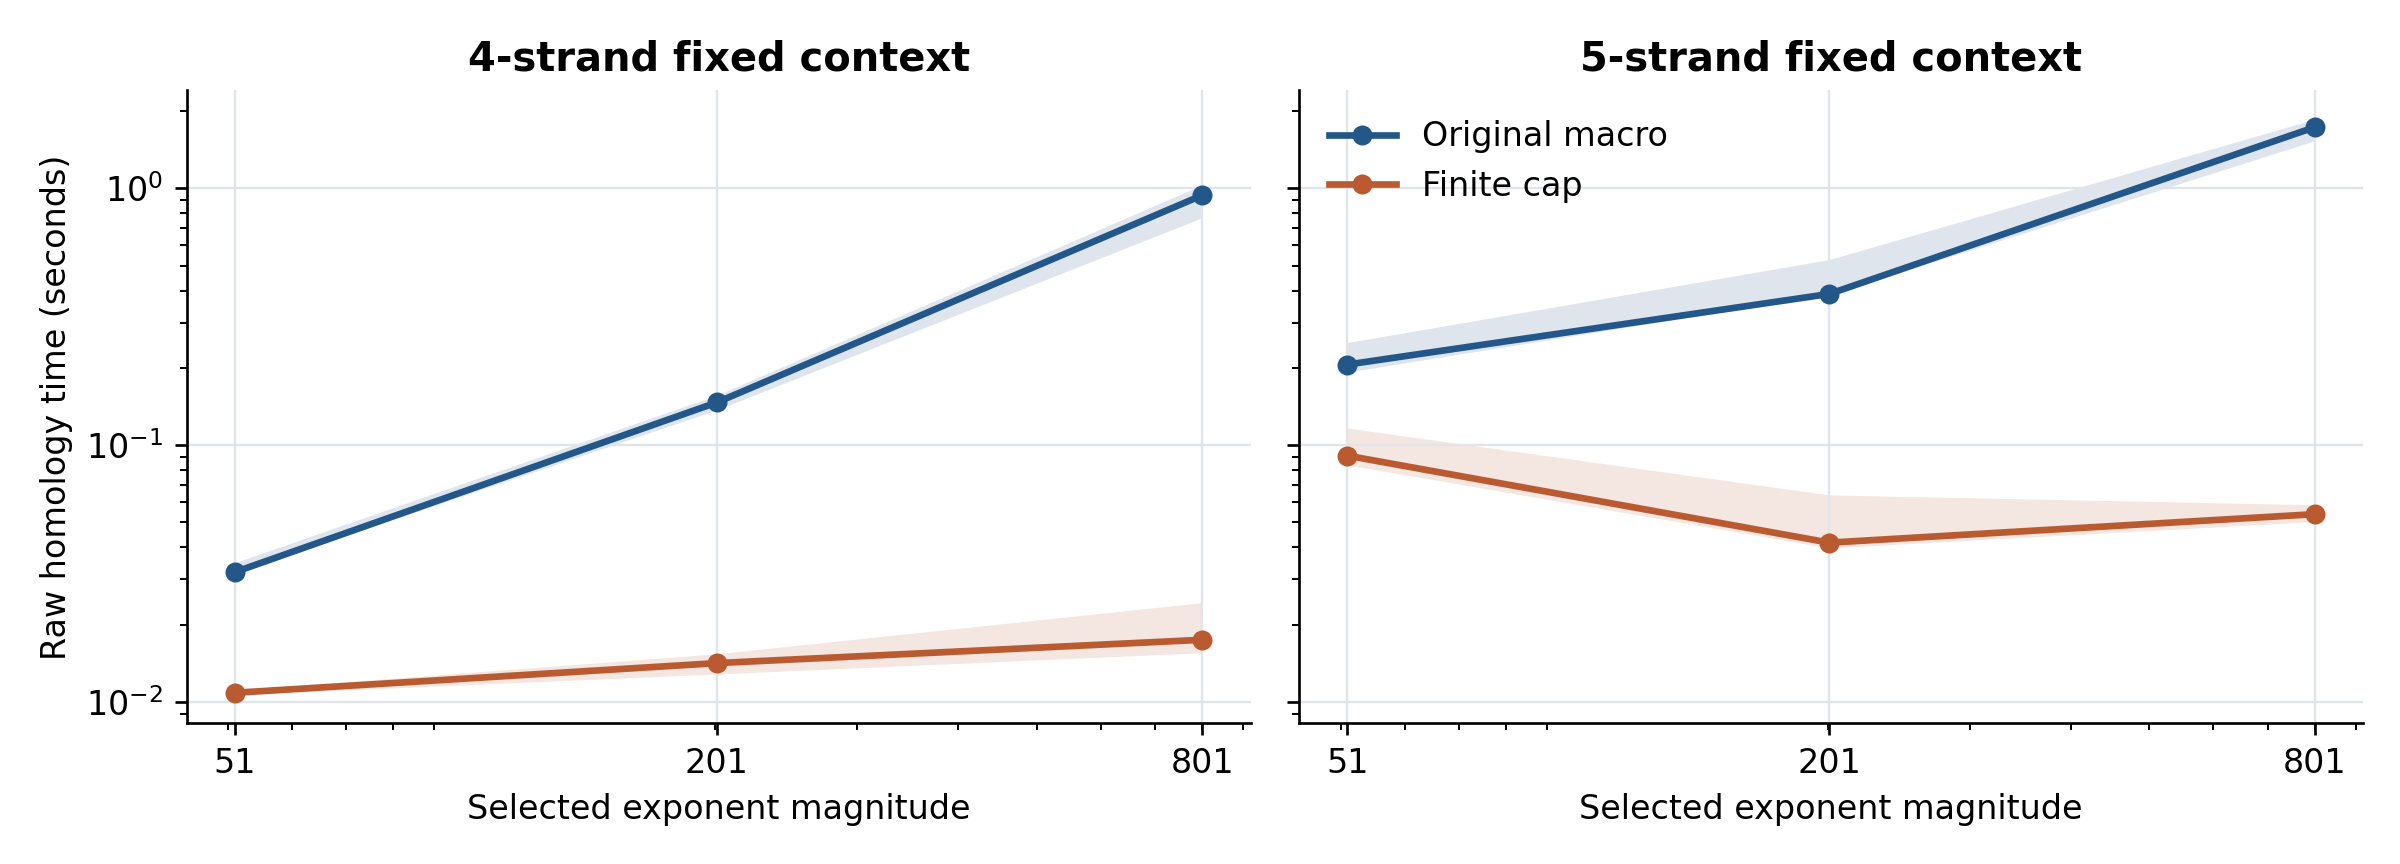
\includegraphics[width=\textwidth]{figures/tail_timings.png}
\caption{Median raw homology time for fixed contexts; shading spans the first and third quartiles of seven samples. The original macro construction grows with the selected exponent; the cap calculation uses the same finite complex. Both axes are logarithmic.}
\label{fig:tailtime}
\end{figure}

A more informative exact-size example uses
\[
 \sigma_2^{-1}\sigma_1\sigma_2\sigma_3^M
 \sigma_2^{-1}\sigma_1\sigma_3^{-1},\qquad M=10^{100}+1.
\]
Here $L=6$, the cap is eight, and $\nu=3$. The result has total rank
\[
 3M-2=3\cdot10^{100}+1,
\]
represented by eleven exceptional points and one constant interval, using 1,650 basis elements. The recorded calculation takes about $0.035$ seconds including $d^2$ and $A^2$ checks. This time is illustrative; the exact finite representation is the substantive result. The cap is a two-component link while the original closure is a knot, demonstrating why the component check must refer to the original exponent.

All these long-tail knots are structurally easy for the maintained recognizer. The finite-cap result accelerates their \emph{requested exact homology}; it is not a measured improvement on hard unknot decisions. Report 14's earlier interval experiment imposed a common matching and common square-zero coefficient on an entire connected differential summand. The present argument instead uses a full matrix $A$ containing arbitrary fixed-context state maps, and the examples above are actual braid closures. The wider applicability of this closed-complex calculation does not make it a relative-boundary replacement.

\subsection{Direct structural evaluation on run input}
The supplied balanced example is the five-strand closure
\[
 \sigma_1^M\sigma_2^{-M}\sigma_3^M\sigma_4^{-M},\qquad M=10^{100}+1.
\]
Its writhe is zero and none of its four runs dominates the rest. The signed Seifert graph is homogeneous, with canonical genus $2M-2=2\cdot10^{100}$. The succinct front end certifies nontriviality directly. This illustrates an improvement in the representation accepted by the implementation, using an existing topological criterion.
A focused interface benchmark uses this same four-run family with magnitudes
101, 1,001, and 10,001. Each arm starts with the identical already parsed run
tuple. The expanded arm includes letter expansion, fresh PD construction and
validation, and the maintained Seifert certificate; the direct arm evaluates
the signed-run certificate. The latter batches 100 fresh calls per sample.
Seven shuffled paired rounds include an expanded A/A arm. Every common
certificate field agrees, and all 2,100 direct certificates pass independent
verification outside the timers.
\begin{table}[htbp]
\centering\small
\begin{tabular}{@{}rrrrr@{}}
\toprule
Magnitude & Crossings & Expanded (ms) & Direct ($\mu$s) & A/A \\
\midrule
101 & 404 & 4.787 & 5.971 & 1.053 \\
1,001 & 4,004 & 48.083 & 5.039 & 1.039 \\
10,001 & 40,004 & 484.068 & 4.482 & 0.958 \\
\bottomrule
\end{tabular}

\caption{Structural certificate evaluation from the same run input. Note the
different time units. These timings include the representation conversion
required by the expanded route and do not measure the full recognition portfolio.}
\label{tab:structural}
\end{table}
The direct call takes roughly five microseconds at these sizes while the
expanded route grows from about five to 484 milliseconds. The input has four
runs throughout; this measures the work avoided by the representation change.
The shared environment included a concurrent regression run, recorded in the
raw JSON. The exact timings and especially very large ratios should therefore
be read as interface measurements, not transferable hardware constants.


\subsection{Reproduction and integration}
Run the following from the archive root to execute the complete integrated suite and the separate mathematical checks:
\begin{lstlisting}[language=bash]
python tools/verify_all.py
\end{lstlisting}
The benchmark commands are separate, so reproducing correctness does not silently replace the delivered measurements. The top-level README gives all commands, input conventions, evidence paths, and the patch workflow. For example:
\begin{lstlisting}[language=bash]
cd implementation/fast
python -m fastunknot khovanov examples/conway.json \
  --reduction graded-adaptive
python -m fastunknot.symbolic_braid \
  ../../examples/four_strand_tail.json --mode homology --check-d2
python -m fastunknot.symbolic_braid \
  ../../examples/balanced_four_runs.json --mode certificate
\end{lstlisting}
The article rebuild script invokes \code{pdflatex} until references stabilize, using the delivered tables and figure. A separate evidence-refresh script can regenerate them from a new run's JSON. The patch is checked against the exact baseline and can be reviewed before application; the runnable proposed source tree is included for inspection without patching a working checkout.



\section{A more precise geometric route to quasi-polynomial time}
\label{sec:geometry}

\subsection{What the current primary source already provides}
Lackenby's July 2026 preprint is more informative than the early talk alone. Proposition 9.1 bounds the number of iterations by $\ell(g+1)^\ell$, and Proposition 10.2 bounds hierarchy length linearly in initial handle complexity. When an essential hierarchy exists, Theorem 14.1 supplies an efficiently encoded hierarchy with polynomial verification. Theorem 14.4 supplies compressed cutting for handle structures of uniform type, including parallelity-bundle type and attachment information, polynomial in handle count and logarithmic \emph{extended} surface weight. Proposition 14.2 supplies associated cleanup under its stated hypotheses, including irreducibility, an essential boundary pattern, and a connected normal cutting surface \cite{lackenby2026}. These hypotheses must be maintained through intermediate operations.

Thus it would be inaccurate to say that no compressed-cutting theorem exists. Section 9 of the preprint itself observes that some steps are not yet specified precisely enough for a time estimate. What is still missing from this implementation is the constructive full hierarchy discovery and repair process with bounded cumulative work and encoded representations. Polynomial certificate verification is not polynomial discovery.

\subsection{Separate deterministic depth from interacting repairs}
The \code{openai/math} repository suggests a useful counting principle in its mean-payoff-game manuscript: a recursion may have polynomial path length, while only logarithmically many edges use a decreasing branch budget. The manuscript explicitly connects this to reduced-precision recursion in parity games; we need only the elementary counting argument, not the manuscript's headline theorem \cite{openai104,parys}.

\begin{proposition}[One continuing child]
\label{prop:tree}
Suppose a rooted computation tree has height at most $H$. Each node has at most one child preserving a nonnegative integer budget and at most $s$ other children decreasing it; no edge increases it. Starting from budget $B$, the number of nodes is at most
\begin{equation}
 \sum_{j=0}^{\min(B,H)}s^j\binom{H+1}{j+1}.
 \label{eq:tree}
\end{equation}
If $H,s$ are polynomial in input size and $B=O(\log n)$, this is $n^{O(\log n)}$.
\end{proposition}
\begin{proof}
At depth $h$, choose the $j$ positions of budget-decreasing edges and then at most $s$ labels at each such position. All other edges have at most one choice. This gives at most $\binom hj s^j$ nodes. Sum over $h$ and use $\sum_{h=j}^H\binom hj=\binom{H+1}{j+1}$. The asymptotic bound follows by taking logarithms.
\end{proof}
The budget must be independently defined from the input and verified along actual operations. Choosing a distinguished child retrospectively from an unknown computation tree is not an algorithmic bound.

\subsection{An exact dependency-graph bound}
\begin{theorem}[Acyclic repairs]
\label{thm:repairs}
Let $D$ be a fixed finite directed acyclic graph on $\ell$ modules. Module $i$ carries an integer counter $0\le x_i\le g_i$. Each event strictly decreases its distinguished counter $x_i$, and may increase other counters only at out-neighbors of $i$. Labels, bounds, and $D$ are fixed. Then the number of events is at most
\begin{equation}
 R(D,\mathbf g)=\sum_{\pi}\prod_{v\in\pi}g_v,
 \label{eq:pathsum}
\end{equation}
where the sum runs over all nonempty directed paths, including one-vertex paths. If the maximum outdegree is $d$, every path has at most $B$ edges, and $g_i\le g$, then
\begin{equation}
 R(D,\mathbf g)\le \ell g\sum_{k=0}^B(dg)^k.
 \label{eq:repairqp}
\end{equation}
\end{theorem}
\begin{proof}
Let $r_i$ count events distinguished at $i$. Partition the run into intervals between events at predecessors of $i$. During an interval its counter cannot increase, so at most $g_i$ events at $i$ occur. Therefore
\[
 r_i\le g_i\left(1+\sum_{j\to i}r_j\right).
\]
Induction in topological order expands this recurrence into the sum of products over all paths ending at $i$. Summing gives \eqref{eq:pathsum}. There are at most $\ell d^k$ paths with $k$ edges, and their products are at most $g^{k+1}$, giving \eqref{eq:repairqp}.
\end{proof}

The weighted sum is computed by a single topological pass. Its numerical value can be enormous, but its bit length is polynomial in the number of vertices and the encoded counter bounds. That does not make the number of events polynomial: the numerical $g$, not merely $\log g$, must be controlled in \eqref{eq:repairqp}.

For common $g$, an edgeless graph gives $\ell g$; a complete acyclic graph gives $(g+1)^\ell-1$; and a directed chain gives $\sum_{k=1}^{\ell}(\ell-k+1)g^k$. A low edge count alone is insufficient. Conversely, $\ell,d,g=n^{O(1)}$ and $B=O(\log n)$ give a quasi-polynomial number of charged events even with $\ell=\Theta(n)$ modules. A total-work bound additionally requires controlled per-event bit cost, uncharged operations, and intermediate representation size. This is a more flexible research target than literally requiring only logarithmically many cuts.

\subsection{The topological obligation is substantial}
Disjoint local cutting operations commute when their collars, embeddings, and attachment data are explicitly transported through the common complement of a repair neighborhood. This observation can preserve unaffected geometric data. It does not automatically preserve the predicates used to select a surface: nonseparatingness, homology constraints, or globally optimized choices can depend on remote regions. A sound dependency graph must include dependencies of those certificates as well as intersections of geometric supports.

Later hierarchy surfaces also need not be properly embedded surfaces in the original manifold; their boundaries can lie on earlier cut faces. Therefore a commutation argument must specify the agreement maps between the appropriate intermediate manifolds. Neither a planar metric embedding nor a small graph separator supplies that data. The theorem above is an exact abstraction and a testable target for a future implementation, not a property we assume of Lackenby's algorithm.

\section{Research questions with concrete next steps}
\label{sec:future}
\begin{enumerate}[label=\textbf{\arabic*.},itemsep=6pt]
\item \textbf{Control graded transfer fill.} Can the scalar contraction be selected to minimize the support of the lifted representatives and of $D$, while retaining the $S E_\delta$ composition bound? Record binary incidences and downstream entry growth, not just pivots removed. A useful result would be a structural bound for contractions produced by actual crossing extension.
\item \textbf{Make the adaptive choice quantitative.} Compare a cheap estimate of $S$, $E_\delta$, and binary block dimensions with the remaining sparse Schur work. Prove a competitive overhead bound for the switch, including a failed expensive prediction. The present threshold is inherited engineering policy, not an optimality theorem.
\item \textbf{Store the contraction as a reusable circuit.} Instead of expanding all of $D$, can one carry a straight-line representation of $P\delta(1+H_0\delta)^{-1}I$ through subsequent crossings and decide the final rank with controlled circuit growth? The critical question is the cost of composition and equality of the represented maps, not the existence of a compact formula.
\item \textbf{Compress several long runs simultaneously.} The one-tail construction works because sufficiently high degree sees one fixed finite matrix. With multiple independently long runs, determine the finite chambers, boundary interfaces, and matrix families that govern the answer. A valid algorithm must handle mixed context differentials and cannot independently shorten runs using the other runs' original expanded lengths.
\item \textbf{Replace raw context length by certified homological span.} If the surrounding tangle can be reduced, relative to its boundary, to a complex of span $w$, can the finite-tail cap be lowered to $w+2$? The repeated saddle and dot natural transformations must be transported through that same reduction. Separate homology calculations of closed states do not preserve the interface data required by the proof. An effective construction could bring some balanced, structurally inconclusive families within reach.
\item \textbf{Address the structural exclusion.} Every eligible dominant-run knot is already detected by the signed Seifert interval. Identify repetition patterns among the residual nonhomogeneous braids for which that interval contains zero. Without this step, further dramatic long-twist timings may have little effect on unknot recognition.
\item \textbf{Restore quantum information where useful.} The transfer already retains $q$, while the twist macro output intentionally forgets it. Develop exact compact bidegree profiles, with the correct alternating local twist maps if coefficients change. Prove representation bounds before advertising quantum-graded output.
\item \textbf{Implement compressed cutting with attachments.} Use the existing normal-surface primitive from the current literature and retain the actual attaching information, parallelity-bundle type, and provenance. A fast orbit count alone does not reconstruct a cut manifold.
\item \textbf{Measure certified repair dependencies.} Instrument a genuine geometric algorithm so every repair declares which stored geometry and which global predicates it invalidates. Measure the longest dependency path, counter ranges, and binary representation sizes. The conditions of Theorem~\ref{thm:repairs} must be checked against these records.
\item \textbf{Find an input-bounded mass for side repairs.} Allow one deterministic continuation but force every other branch to reduce a certified region mass by a fixed factor. Together with polynomial local cost this would activate Proposition~\ref{prop:tree}. Defining mass from the unknown completed run would be circular.
\item \textbf{Build complementary hard benchmarks.} Separate prime nonhomogeneous inputs, hard unknot diagrams, width stress, long-run symbolic homology, dense valid algebra controls, and large normal coordinates. Report which earlier stage decides each instance. A benchmark collection should expose the unresolved state-volume mechanism, not only easy families with large crossing counts.
\end{enumerate}

\section{Conclusions}
The grading supplies a fully constructive transfer of the residual differential, including the maps that a survivor count cannot determine. A long signed twist admits an exact finite computation and compact full homological-degree output, with an explicit binary-input bound. The accompanying dominance argument also identifies why this appealing family does not test the hardest part of the current recognizer: its knots already satisfy the structural certificate. Succinct signed-run evaluation improves that interface directly.

These are precise additions to the research program. They preserve the distinction between a fast primitive, a compressed representation, a useful recognition family, and a global complexity theorem. Achieving general quasi-polynomial unknot recognition still requires control of the executed state volume or a constructive geometric hierarchy whose cumulative repair and representation costs satisfy a proved bound.

\clearpage
\begingroup
\small
\begin{thebibliography}{99}
\raggedright
\bibitem{proveit} V. Reshetnikov, \emph{ProveIt, Topology/UnknotRecognition}, source snapshot \code{d54009df0ea3751b8662bb76549d3c1bb0eec19c}, 8 October 2026. \url{https://github.com/VladimirReshetnikov/ProveIt/tree/d54009df0ea3751b8662bb76549d3c1bb0eec19c/Topology/UnknotRecognition}.
\bibitem{barnatan} D. Bar--Natan, \emph{Khovanov's homology for tangles and cobordisms}, Geometry \& Topology 9 (2005), 1443--1499. \url{https://arxiv.org/abs/math/0410495}.
\bibitem{fastkh} D. Bar--Natan, \emph{Fast Khovanov homology computations}, Journal of Knot Theory and Its Ramifications 16 (2007), 243--255. \url{https://arxiv.org/abs/math/0606318}.
\bibitem{km} P. B. Kronheimer and T. S. Mrowka, \emph{Khovanov homology is an unknot-detector}, Publications Math\'ematiques de l'IH\'ES 113 (2011), 97--208. \url{https://arxiv.org/abs/1005.4346}.
\bibitem{real} P. Real, \emph{Homological perturbation theory and associativity}, Homology, Homotopy and Applications 2 (2000), 51--88. \url{https://projecteuclid.org/journals/homology-homotopy-and-applications/volume-2/issue-1/Homological-perturbation-theory-and-associativity/hha/1139841213.full}.
\bibitem{stosic} M. Sto\v{s}i\'c, \emph{Homological thickness and stability of torus knots}, Algebraic \& Geometric Topology 7 (2007), 261--284. \url{https://arxiv.org/abs/math/0511532}.
\bibitem{watson} L. Watson, \emph{Surgery obstructions from Khovanov homology}, Selecta Mathematica 18 (2012), 417--472, especially Lemma 4.14. \url{https://arxiv.org/abs/0807.1341}.
\bibitem{tagami} K. Tagami, \emph{The behavior of the maximal degree of the Khovanov homology under twisting}, Topology Proceedings 46 (2015), 45--54. \url{https://topology.nipissingu.ca/tp/reprints/v46/tp46005.pdf}.
\bibitem{lobb_twist} A. Lobb, \emph{2-strand twisting and knots with identical quantum knot homologies}, Geometry \& Topology 18 (2014), 873--895. \url{https://arxiv.org/abs/1103.1412}.
\bibitem{cromwell} P. R. Cromwell, \emph{Homogeneous links}, Journal of the London Mathematical Society (2) 39 (1989), 535--552.
\bibitem{lobb} A. Lobb, \emph{Computable bounds for Rasmussen's concordance invariant}, Compositio Mathematica 147 (2011), 661--668. \url{https://arxiv.org/abs/0908.2745}.
\bibitem{abe} T. Abe, \emph{The Rasmussen invariant of a homogeneous knot}, Proceedings of the American Mathematical Society 139 (2011), 2647--2656. \url{https://arxiv.org/abs/1003.5392}.
\bibitem{lackenby2026} M. Lackenby, \emph{Incompressible surfaces, hierarchies and unknot recognition}, July 2026 preprint, arXiv:2607.23350v1. \url{https://arxiv.org/abs/2607.23350}.
\bibitem{openai104} OpenAI, \emph{Deterministic quasipolynomial-time mean-payoff games}, September 2026 research manuscript, section ``Counting calls and bit operations.'' \url{https://github.com/openai/math/blob/main/preprints/Deterministic-quasipolynomial-time-mean-payoff-games-September-25-2026/build/source/sections/06-complexity.tex}. The elementary recursion count is re-proved here; the headline result is not assumed.
\bibitem{parys} P. Parys, \emph{Parity games: Zielonka's algorithm in quasi-polynomial time}, MFCS 2019, LIPIcs 138, 10:1--10:13. \url{https://doi.org/10.4230/LIPIcs.MFCS.2019.10}.
\end{thebibliography}
\endgroup
\end{document}
